\documentclass[12pt]{article} %***
\usepackage[sectionbib]{natbib}
\usepackage{array,epsfig,fancyheadings,rotating}
%\usepackage[]{hyperref}  %<----modified by Ivan
%%%%%%%%%%%%%%%%%%%%%%%%%%%%%%%%%%%%
\usepackage{sectsty, secdot}
%\sectionfont{\fontsize{12}{15}\selectfont}
\sectionfont{\fontsize{12}{14pt plus.8pt minus .6pt}\selectfont}
\renewcommand{\theequation}{\thesection\arabic{equation}}
\subsectionfont{\fontsize{12}{14pt plus.8pt minus .6pt}\selectfont}
%%%%%%%%%%%%%%%%%%%%%%%%%%%%%%%%%%%%%%%%%%%%%%%%%%%%%%%%%%%%%%%%%%%%%%%%%%%%%%%%%%%%%%%%

\textwidth=36pc
\textheight=49pc
\oddsidemargin=1pc
\evensidemargin=1pc
\headsep=15pt
\topmargin=.6cm
\parindent=1.7pc
\parskip=0pt

\usepackage{amsmath}
\usepackage{amssymb}
\usepackage{amsfonts}
\usepackage{multirow}
\usepackage{amsthm}
\usepackage{todonotes}
\usepackage{mathtools}
\usepackage{subcaption}
\usepackage{color}
\usepackage{cite}

\usepackage{xr}
\externaldocument{hyperparam-theory-appendix}


\setcounter{page}{1}
\newtheorem{theorem}{Theorem}
\newtheorem{lemma}{Lemma}
\newtheorem{corollary}{Corollary}
\newtheorem{proposition}{Proposition}
\theoremstyle{definition}
\newtheorem{definition}{Definition}
%\newtheorem{proof}{Proof}
\newtheorem{example}{Example}
\newtheorem{remark}{Remark}
\newtheorem{condition}{Condition}
\newtheorem{assump}{Assumption}
\DeclareMathOperator{\diag}{diag}
\DeclareMathOperator{\spann}{span}
\newcommand{\textred}[1]{\textcolor{red}{#1}}
\pagestyle{fancy}

%%%%%%%%%%%%%%%%%%%%%%%%%%%%%%%%%%%%%%%%%%%%%%%%%%%%%%%%%%%%%%%%%%%%%%%%%%%%%%%%%%%%%%%%%%%%%%%%%%%%%%%%%%%%%%%%%%%%%%%%%%%%
\pagestyle{fancy}
\def\n{\noindent}
\lhead[\fancyplain{} \leftmark]{}
\chead[]{}
\rhead[]{\fancyplain{}\rightmark}
\cfoot{}
%\headrulewidth=0pt  %<-modified by Ivan

%%%%%%%%%%%%%%%%%%%%%%%%%%%%%%%%%%%%%%%%%%%%%%%%%%%%%%%%%%%%%%%%%%%%%%%%%%%%%%%%%%%%%%%%%%%%%%%%%%%%%%%%%%%%%%%%%%%%%%%%%%%%

\DeclareMathOperator*{\argmin}{arg\,min}

%%%%%%%%%%%%%%%%%%%%%%%%%%%%%%%%%%%%%%%%%%%%%%%%%%%%%%%%%%%%%%%%%%%%%%%%%%%%%%%%%%%%%%%%%%%%%%%%%%%%%%%%%%%%%%%%%%%%%%%%%%%%

%\cfoot{\thepage}

\begin{document}

%%%%%%%%%%%%%%%%%%%%%%%%%%%%%%%%%%%%%%%%%%%%%%%%%%%%%%%%%%%%%%%%%%%%%%%%%%%%%%%%%%%%%%%%%%%%%%%%%%%%%%%%%%%%%%%%%%%%%%%%%%%%
%%%%%%%%%%%%%%%%%%%%%%%%%%%%%%%%%%%%%%%%%%%%%%%%%%%%%%%%%%%%%%%%%%%%%%%%%%%%%%%%%%%%%%%%%%%%%%%%%%%%%%%%%%%%%%%%%%%%%%%%%%%%

\renewcommand{\baselinestretch}{2}

\markright{ \hbox{\footnotesize\rm Statistica Sinica
%{\footnotesize\bf 24} (201?), 000-000
}\hfill\\[-13pt]
\hbox{\footnotesize\rm
%\href{http://dx.doi.org/10.5705/ss.20??.???}{doi:http://dx.doi.org/10.5705/ss.20??.???}
}\hfill }

\markboth{\hfill{\footnotesize\rm Jean Feng and Noah Simon} \hfill}
{\hfill {\footnotesize\rm Hyper-parameter selection via split-sample validation} \hfill}

\renewcommand{\thefootnote}{}
$\ $\par

%%%%%%%%%%%%%%%%%%%%%%%%%%%%%%%%%%%%%%%%%%%%%%%%%%%%%%%%%%%%%%%%%%%%%%%%%%%%%%%%%%%%%%%%%%%%%%%%%%%%%%%%%%%%%%%%%%%%%%%%%%%%

\fontsize{12}{14pt plus.8pt minus .6pt}\selectfont \vspace{0.8pc}
\centerline{\large\bf An analysis of the cost of hyper-parameter selection via split-}
\vspace{2pt} \centerline{\large\bf sample validation, with applications to penalized regression}
\vspace{.4cm} \centerline{Jean Feng, Noah Simon} \vspace{.4cm} \centerline{\it
Department of Biostatistics, University of Washington} \vspace{.55cm} \fontsize{9}{11.5pt plus.8pt minus
.6pt}\selectfont

%%%%%%%%%%%%%%%%%%%%%%%%%%%%%%%%%%%%%%%%%%%%%%%%%%%%%%%%%%%%%%%%%%%%%%%%%%%%%%%%%%%%%%%%%%%%%%%%%%%%%%%%%%%%%%%%%%%%%%%%%%%%

\begin{quotation}
\noindent {\it Abstract:}
In the regression setting, given a set of hyper-parameters, a model-estimation procedure constructs a model from training data. The optimal hyper-parameters that minimize generalization error of the model are usually unknown. In practice they are often estimated using split-sample validation. Up to now, there is an open question regarding how the generalization error of the selected model grows with the number of hyper-parameters to be estimated. To answer this question, we establish finite-sample oracle inequalities for selection based on a single training/test split and based on cross-validation. We show that if the model-estimation procedures are smoothly parameterized by the hyper-parameters, the error incurred from tuning hyper-parameters shrinks at nearly a parametric rate. Hence for semi- and non-parametric model-estimation procedures with a fixed number of hyper-parameters, this additional error is negligible. For parametric model-estimation procedures, adding a hyper-parameter is roughly equivalent to adding a parameter to the model itself. In addition, we specialize these ideas for penalized regression problems with multiple penalty parameters. We establish that the fitted models are Lipschitz in the penalty parameters and thus our oracle inequalities apply. This result encourages development of regularization methods with many penalty parameters.
\vspace{9pt}

\noindent {\it Key words and phrases:}
Cross-validation, Regression, Regularization.
\par
\end{quotation}\par

\def\thefigure{\arabic{figure}}
\def\thetable{\arabic{table}}

\renewcommand{\theequation}{\thesection.\arabic{equation}}



\fontsize{12}{14pt plus.8pt minus .6pt}\selectfont

\setcounter{section}{1} %***
\setcounter{equation}{0} %-1

\section{Introduction}

%JF wow this paper's english can really use some level-upping. some paragraphs also don't flow.
%JF clean up notation - bold symbols appropriately too!
% sort out T vs D^{(n_T)}

Per the usual regression framework, suppose we observe response $y \in \mathbb{R}$ and predictors $\boldsymbol {x} \in \mathbb{R}^p$. Suppose $y$ is generated by a true model $g^*$ plus random error $\epsilon$ with mean zero, e.g.
$y = g^*(\boldsymbol x) + \epsilon$.
Our goal is to estimate $g^*$.
Many model-estimation procedures can be formulated as selecting a model from some function class $\mathcal{G}$ given training data $T$ and $J$-dimensional hyper-parameter vector $\boldsymbol{\lambda}$. For example, in penalized regression problems, the fitted model can be expressed as the minimizer of the penalized training criterion
\begin{equation}
\label{eq:intro_pen_reg}
\hat{g}(\boldsymbol \lambda | T) = \argmin_{g\in \mathcal{G}} \sum_{(\boldsymbol{x}_i, y_i) \in T} \left (y_i -  g(\boldsymbol{x}_i) \right )^2 + \sum_{j=1}^J \lambda_j P_j(g),
\end{equation}
%JF:  I would like to divide by number of obs in T
where $P_j$ are penalty functions and $\lambda_j$ are penalty parameters that serve as hyper-parameters of the model-estimation procedure.

If $\Lambda$ is a set of possible hyper-parameters, the goal is to find a penalty parameter $\boldsymbol{\lambda} \in \Lambda$ that minimizes the expected generalization error
$
\mathbb{E} \left [
\left ( y - \hat{g}(\boldsymbol{\lambda} | T)(\boldsymbol{x}) \right )^2
\right ].
$
Typically one uses a sample-splitting procedure where models are trained on a random partition of the observed data and evaluated on the remaining data.
One then chooses the hyper-parameter $\hat{\boldsymbol{\lambda}}$ that minimize the error on this validation set.
For a more complete review of cross-validation, refer to \citet{arlot2010survey}.

The performance of split-sample validation procedures is typically characterized by an oracle inequality that bounds the generalization error of the expected model selected from the validation set procedure. For $\Lambda$ that are finite, oracle inequalities have been established for a single training/validation split \citep{gyorfi2006distribution} and a general cross-validation framework \citep{van2003unified, van2004asymptotic}. To handle $\Lambda$ over a continuous range, one can use entropy-based approaches \citep{lecue2012oracle}.
%JF: I would like to add reasons for why we want to think about a continuous range because people don't typically think about this.

The goal of this paper is to characterize the performance of models when the hyper-parameters are tuned by some split-sample validation procedure. We are particularly interested in an open question raised in \citet{bengio2000gradient}: what is the ``amount of overfitting... when too many hyper-parameters are optimized''? In addition, how many hyper-parameters is ``too many''? In this paper we show that actually a large number of hyper-parameters can be tuned without overfitting. In fact, if an oracle estimator converges at rate $R(n)$, then the number of hyper parameters $J$ can grow at roughly a rate of $J = O_p(nR(n))$ up to log terms without affecting the convergence rate. In practice, for penalized regression, this means that one can propose and tune over much more complex models than are currently often used.

To show these results, we prove that finite-sample oracle inequalities of the form
\begin{equation}
\label{thrm:intro_oracle_ineq}
\mathbb{E} \left [
\left ( y - \hat{g}(\hat{\boldsymbol{\lambda}} | T)(\boldsymbol{x}) \right )^2
\right ]
\le
(1+a)
\underbrace{
	\inf_{\lambda \in \Lambda}
	\mathbb{E} \left [
	\left ( y - \hat{g}(\boldsymbol{\lambda} | T)(\boldsymbol{x}) \right )^2
	\right ]
}_{\text{Oracle risk}}
+ \delta \left(J,n\right)
\end{equation}
are satisfied with high probability for some constant $a \ge 0$ and remainder $\delta(J,n)$ that depends on the number of tuned hyper-parameters $J$ and the number of samples $n$.
Under the assumption that the model -estimation procedure is Lipschitz in the hyper-parameters, we find that $\delta$ scales linearly in $J$.
For parametric model-estimation procedures, the additional error from tuning hyper-parameters is roughly $O_p(J/n)$, which is similar to the typical parametric model-estimation rate $O_p(p/n)$ where the model parameters are not regularized.
For semi- and non-parametric model-estimation procedures, this error is generally dominated by the oracle risk so we can actually grow the number of hyper-parameters without affecting the asymptotic convergence rate.

In addition, we specialize our results to penalized regression models of the form \eqref{eq:intro_pen_reg}.
The models in our examples are Lipschitz so that our oracle inequalities apply.
%Again, we find that additional penalty parameters only add a near-parametric error term, which has a negligible effect in semi- and non-parametric settings.
This suggests that multiple penalty parameters may improve the model estimation and that the recent interest in combining penalty functions (e.g. elastic net and sparse group lasso \citep{zou2003regression, simon2013sparse}) may have artificially restricted themselves to two-way combinations.

During our literature search, we found few theoretical results relating the number of hyper-parameters to the generalization error of the selected model. 
Much of the previous work only considered tuning a one-dimensional hyper-parameter over a finite $\Lambda$, proving asymptotic optimality \citep{van2004asymptotic} and finite-sample oracle inequalities \citep{van2003unified, gyorfi2006distribution}. Others have addressed split-sample validation for specific penalized regression problems with a single penalty parameter, such as linear model selection \citep{li1987asymptotic, shao1997asymptotic, golub1979generalized, chetverikov2016cross, chatterjee2015prediction}.
Only the results in \citet{lecue2012oracle} are relevant to answering our question of interest. A potential reason for this dearth of literature is that, historically, tuning multiple hyper-parameters was computationally difficult.
However there have been many recent proposals that address this computational hurdle \citep{bengio2000gradient, foo2008efficient, snoek2012practical}.

Section \ref{sec:main_results} presents oracle inequalities for sample-splitting procedures to understand how the number of hyper-parameters affects the model error.
Section \ref{sec:examples} applies these results to penalized regression models.
Section \ref{sec:simulations} provides a simulation study to support our theoretical results.
Oracle inequalities for general model-estimation procedures and proofs are given in the Supplementary Materials.



\section{Oracle Inequalities} \label{sec:main_results}

Here we establish oracle inequalities for models where the hyper-parameters are tuned by a single training/validation split and cross-validation.
We are interested in studying model-estimation procedures that vary smoothly in their hyper-parameters; such procedures tend to be easier to use and therefore tend to be more popular.
%\textcolor{red}{(Too dense too early --- also do these need $n_T$ super scripts? Or can they all just be $n$?)}
%\textcolor{red}{Jean: is this better?}


Let $D^{(n)}$ denote a dataset with $n$ samples.
Given dataset training data $D^{(m)}$, let $\hat{g}^{(m)}(\boldsymbol{\lambda} | D^{(m)})$ be some model-estimation procedure that maps hyper-parameter $\boldsymbol{\lambda}$ to a function in $\mathcal{G}$.
We assume the following Lipschitz-like assumption on the model-estimation procedure.
In particular, we suppose that for any $\boldsymbol{x}$, the predicted value $\hat{g}^{(m)}(\boldsymbol{\lambda} | D^{(m)})(\boldsymbol{x})$ is Lipschitz in $\boldsymbol{\lambda}$:
\begin{assump}
	\label{assump:lipschitz}
	Suppose there is a set $\mathcal{X}^{(L)} \subseteq \mathcal{X}$ such that for any $n_T \in \mathbb{N}$ and dataset $D^{(n_T)}$, there is a function $C_\Lambda(\boldsymbol{x} | D^{(n_T)}) : \mathcal{X}^{(L)} \mapsto \mathbb{R}^+$ such that for any $\boldsymbol{x} \in \mathcal{X}^{(L)}$, we have for all $\boldsymbol{\lambda}^{(1)}, \boldsymbol{\lambda}^{(2)} \in \Lambda$
	\begin{align}
	\left |
	\hat{g}^{(n_T)}(\boldsymbol{\lambda}^{(1)}|D^{(n_T)})(\boldsymbol{x}) - \hat{g}^{(n_T)}(\boldsymbol{\lambda}^{(1)}|D^{(n_T)})(\boldsymbol{x}) \right |
	\le C_\Lambda(\boldsymbol{x}|D^{(n_T)}) \|\boldsymbol{\lambda}^{(1)} - \boldsymbol{\lambda}^{(2)}\|_2.
	\end{align}
\end{assump}
\noindent We provide examples of penalized regression models that satisfy this assumption in Section \ref{sec:examples}.
%From this Lipschitz assumption, we find that the error from tuning multiple hyper-parameters shrinks at roughly a parametric rate of $O_p(J/n_V)$.
%JF removing sentences cause it seems repetitive
%Hence for semi- and non-parametric model-estimation procedures, the error from tuning a fixed number of hyper-parameters is negligible.
%Moreover, we can specify an upper bound on the rate at which the number of hyper-parameters can grow without asymptotically increasing the generalization error of the selected model.

\subsection{A Single Training/Validation Split}\label{sec:single}

In the training/validation split procedure, the dataset $D^{(n)}$ is randomly partitioned into a training set $T = (X_T, Y_T)$ and validation set $V = (X_V, Y_V)$ with $n_T$ and $n_V$ observations, respectively.
The selected hyper-parameter $\hat{\boldsymbol{\lambda}}$ is a minimizer of the validation loss
\begin{equation}
\label{eq:train_val_lambda}
\hat{\boldsymbol \lambda} \in \argmin_{\boldsymbol{\lambda} \in\Lambda} \frac{1}{2} \left \| y-\hat{g}^{(n_T)}( \boldsymbol \lambda | T) \right \|_{V}^{2}
\end{equation}
where $\| h \|^2_{V} \coloneqq \frac{1}{n_V}\sum_{(x_i, y_i)\in V} h^2(x_i, y_i)$ for function $h$.

We now present a finite-sample oracle inequality for the single training/validation split assuming Assumption~\ref{assump:lipschitz} holds.
Our oracle inequality is sharp, i.e. $a=0$ in \eqref{thrm:intro_oracle_ineq}, unlike most other work \citep{gyorfi2006distribution, lecue2012oracle, van2003unified}.
Note that the result below is a special case of Theorem \ref{thrm:train_val_complicated} in Supplementary Materials \ref{appendix:train_val}, which applies to general model-estimation procedures.
\begin{theorem}
	\label{thrm:train_val}
	Let $\Lambda=[\lambda_{\min},\lambda_{\max}]^{J}$ where $\Delta_{\lambda} = \lambda_{\max} - \lambda_{\min} \ge 0$.
	Suppose random variables $\epsilon_i$ from the validation set $V$ are independent with expectation zero and are uniformly sub-Gaussian with parameters $b$ and $B$:
	$$
	\max_{i: (x_i, y_i) \in V} B^2 \left ( \mathbb{E} e^{|\epsilon_i|^2/B^2} - 1 \right ) \le b^2.
	$$
%	Let training data $T$ and the covariates of the validation set $X_V$ be fixed.
	Let the oracle risk be denoted
	\begin{equation}
	\tilde{R}(X_V|T) = \argmin_{\lambda \in \Lambda} \left \| g^*-\hat{g}^{(n_T)}( \boldsymbol{\lambda} | T) \right \|_{V}^{2}.
	\label{eq:tilde_lambda_def}
	\end{equation}
	Suppose Assumption~\ref{assump:lipschitz} is satisfied over the set $X_V$.
	Then there is a constant $c>0$ only depending on $b$ and $B$ such that for all $\delta$ satisfying
	\begin{equation}
	\delta^{2}
	\ge
	c \left (
	\frac{J \log(\|C_\Lambda(\cdot |T)\|_V \Delta_{\Lambda} n + 1)}{n_{V}}
	\vee 
	\sqrt{\frac{J \log(\|C_\Lambda(\cdot |T)\|_V \Delta_{\Lambda} n + 1)}{n_{V}}
		\tilde{R}(X_V|T)}
	\right )
	\label{thrm:train_val_delta}
	\end{equation}
	we have
	\begin{align}
	Pr\left(
	\left\Vert g^* - \hat{g}^{(n_T)}( \hat{\boldsymbol{\lambda}} | T) \right\Vert _{V}^2 -
	\tilde{R}(X_V|T)
	\ge\delta^2
	\middle | 
	T, X_V
	\right )
	&\le c\exp\left(-\frac{n_{V}\delta^{4}}{c^{2} \tilde{R}(X_V|T)}\right)
	+ c\exp\left(-\frac{n_{V}\delta^{2}}{c^{2}}\right).
	\end{align}
	
\end{theorem}
\noindent
Theorem \ref{thrm:train_val} states that with high probability, the excess risk, e.g. the error incurred during the hyper-parameter selection process, is no more than $\delta^2$.
As seen in \eqref{thrm:train_val_delta}, $\delta^2$ is the maximum of two terms: a near-parametric term and the geometric mean of the near-parametric term and the oracle risk. To see this more clearly, we express Theorem \ref{thrm:train_val} using asymptotic notation.
\begin{corollary}
	\label{corr:train_val}
	Under the assumptions given in Theorem \ref{thrm:train_val}, we have
	\begin{align}
	\left\Vert g^* - \hat{g}^{(n_T)}( \hat{\boldsymbol{\lambda}} | T) \right\Vert _{V}^2 &
	\le \min_{\lambda \in \Lambda} \left\Vert g^* - \hat{g}^{(n_T)}( {\boldsymbol{\lambda}} | T) \right \Vert^2_{V}
	\label{eq:asym_train_val_oracle_risk}
	\\
	& + O_p \left(\frac{J\log (n \|C_\Lambda\|_V \Delta_{\Lambda} )}{n_{V}} \right) 
	\label{eq:asym_train_val_theorem1} \\
	& + O_p \left(
	\sqrt{
		\frac{J \log (n \|C_\Lambda\|_V \Delta_{\Lambda} )}{n_{V}}
		\min_{\lambda \in \Lambda} \left\Vert g^* - \hat{g}^{(n_T)}( {\boldsymbol{\lambda}} | T) \right \Vert^2_{V}
	}
	\right ).
	\label{eq:asym_train_val_theorem2}
	\end{align}
\end{corollary}
\noindent
Corollary \ref{corr:train_val} show that the risk of the selected model is bounded by the oracle risk, the near-parameteric term \eqref{eq:asym_train_val_theorem1}, and the geometric mean of the two values \eqref{eq:asym_train_val_theorem2}.
We refer to \eqref{eq:asym_train_val_theorem1} as near-parametric because the error term in (un-regularized) parametric regression models is typically $O_p(J/n)$, where $J$ is the parameter dimension and $n$ is the number of training samples. Analogously, \eqref{eq:asym_train_val_theorem1} is $O_p(J/n_V)$ modulo a $\log n$ term in the numerator.
The geometric mean \eqref{eq:asym_train_val_theorem2} can be thought of as a consequence of tuning hyper-parameters over
\begin{equation}
\mathcal{G}(T) = \left \{ \hat{g}^{(n_T)}( {\boldsymbol{\lambda}}| T) : \boldsymbol{\lambda} \in \Lambda \right \}.
\end{equation}
As $\mathcal{G}(T)$ does not (or is very unlikely to) contain the true model $g^*$, tuning the hyper-parameters via training/validation split is tuning over a the misspecified model class.
The geometric mean takes into account this misspecification error.

In the semi- and non-parametric regression settings, the oracle error usually shrinks at a rate of $O_p(n_T^{-\omega})$ where $\omega \in (0, 1)$.
If the number of hyper-parameters is fixed and $n$ is large, the oracle risk will tend to dominate the upper bound.
Hence for such problems, we can actually let the number of hyper-parameters grow -- the asymptotic convergence rate of the upper bound will be unchanged as long as $J$ grows no faster than
$
O_p\left (
\frac{n_{V} n_T^{-\omega}}{\log (n \|C_\Lambda\|_V \Delta_{\Lambda})}
\right ).
$

\subsection{Cross-Validation}\label{sec:cv}

Now we give an oracle inequality for $K$-fold cross-validation.
Previously, the oracle inequality was with respect to the $L_2$-norm over the validation covariates.
Now we give our result with respect to the functional $L_2$-norm.
We suppose our dataset is composed of independent identically distributed observations $(X,y)$ where $X$ is independent of $\epsilon$.
The functional $L_2$-norm is defined as
$
\left \| h \right \|^2_{L_2} = \int \left |h(x) \right |^2 d\mu(x)
$.

For $K$-fold cross-validation, we randomly partition the dataset $D^{(n)}$ into $K$ sets, which we assume to have equal size for simplicity. Partition $k$ will be denoted $D_k^{(n_V)}$ and its complement will be denoted $D_{-k}^{(n_T)} = D^{(n)} \setminus D_k^{(n_V)}$. We train our model using $D_{-k}^{(n_T)}$ for $k=1,...,K$ and select the hyper-parameter that minimizes the average validation loss
\begin{eqnarray}
\label{kfold_opt}
\hat{\boldsymbol \lambda} &=& \argmin_{\boldsymbol{\lambda} \in\Lambda} \frac{1}{K} \sum_{k=1}^K  \left \| y-\hat{g}^{(n_T)}(\boldsymbol \lambda | D_{-k}^{(n_T)}) \right \|_{D_k^{(n_V)}}^{2}.
\end{eqnarray}

In traditional cross-validation, the final model is retrained on all the data with $\hat{\boldsymbol{\lambda}}$. However bounding the generalization error of the retrained model requires additional regularity assumptions \citep{lecue2012oracle}. We consider the ``averaged version of $K$-fold cross-validation'' instead
\begin{equation}
\label{thrm:avg_cv}
\bar{g}\left ( {D^{(n)}} \right ) = 
\frac{1}{K} \sum_{k=1}^K 
\hat{g}^{(n_T)} \left (\hat{\boldsymbol \lambda} \middle | D^{(n_T)}_{-k} \right ).
\end{equation}
To bound the generalization error of \eqref{thrm:avg_cv}, we require an assumption in \citet{lecue2012oracle} that controls the tail behavior of the fitted models.
A classical approach for bounding the tail behavior of random variable $X$ is to bound its Orlicz norm 
$\|X\|_{L_{\psi_1}}= \inf \{C > 0: \mathbb{E}\exp(|X|/C) - 1 \le 1\}$ \citep{van1996weak}.
\begin{assump}
	\label{assump:tail_margin}
	There exist constants $K_0, K_1 \ge 0$ and $\kappa \ge 1$ such that for any $n_T \in \mathbb{N}$, dataset $D^{(n_T)}$, and $\boldsymbol{\lambda} \in \Lambda$, we have
	\begin{align}
	\left \|
	\left(
	y - \hat{g}^{(n_T)}(\boldsymbol{\lambda} | D^{(n_T)})
	\right)^2
	- \left(
	y - g^*
	\right)^2
	\right \|_{L_{\psi_1}} & \le K_0
	\label{eq:cv_assump1}\\
	\left \|
	\left(
	y - \hat{g}^{(n_T)}(\boldsymbol{\lambda} | D^{(n_T)})
	\right)^2
	- \left(
	y - g^*
	\right)^2
	\right \|_{L_2}
	& \le 
	K_1 \left \|
	g^{*}-\hat{g}(\boldsymbol{\lambda}|D^{(n_{T})})
	\right \|_{L_{2}}^{1/\kappa}.
	\label{eq:cv_assump2}
	\end{align}
\end{assump}

With the above assumption, the following oracle inequality bounds the risk of averaged version of $K$-fold cross-validation.
It is a special case of Theorem~\ref{thrm:jean_cv} in the Supplementary Materials, which extends Theorem 3.5 in \citet{lecue2012oracle}.
The notation $\mathbb{E}_{D^{(m)}}$ indicates the expectation over random $m$-sample datasets $D^{(m)}$ drawn from the probability distribution $\mu$.
\begin{theorem}
	\label{thrm:kfold}
	Let $\Lambda=[\lambda_{\min},\lambda_{\max}]^{J}$ where $\Delta_{\Lambda} = (\lambda_{\max} - \lambda_{\min}) \vee 1$.
	%JF do I really need the \vee above?
	Suppose random variables $\epsilon_i$ are independent with expectation zero, satisfy $\|\epsilon\|_{L_{\psi_2}}= b <\infty$, and are independent of $X$.
	Suppose Assumption~\ref{assump:lipschitz} holds over the set $\mathcal{X}$ and Assumption~\ref{assump:tail_margin} holds.
	Suppose there exists a function $\tilde{h}$ and some $\sigma_0 > 0$ such that
	\begin{align}
	\tilde{h}(n_{T})
	\ge
	1 + \sum_{k=1}^{\infty}
	k\Pr\left(\|C_\Lambda(\cdot |D^{(n_{T})})\|_{L_{\psi_{2}}}\ge2^{k}\sigma_{0}\right).
	\label{eq:prob_bound_cv}
	\end{align}
	Then there exists an absolute constant $c_{1}>0$ and a constant $c_{K_0, b}>0$ such that for any $a > 0$,
	\begin{align}
	\begin{split}
	\mathbb{E}_{D^{(n)}}\left(
	\|
	\bar{g}(D^{(n)})
	-g^{*}
	\|_{L_{2}}^{2}\right)
	& \le	(1+a)
	\inf_{\lambda\in\Lambda}
	\left[\mathbb{E}_{D^{(n_{T})}}\left(\|
	\hat{g}(\boldsymbol{\lambda}|D^{(n_{T})})
	-g^{*}\|_{L_{2}}^{2}\right)\right] \\
	& +
	c_{1}
	\left (\frac{1+a}{a} \right )^2
	\frac{J\log n_{V}}{n_{V}}
	K_0
	\left[\log\left(\Delta_{\Lambda} c_{K_0, b} n \sigma_0 +1\right)+1\right]
	\tilde{h}(n_{T}).
	\end{split}
	\label{eq:cv_lipschitz_oracle_ineq}
	\end{align}
\end{theorem}

As in Theorem \ref{thrm:train_val}, the remainder term in Theorem~\ref{thrm:kfold} includes a near-parametric term $O_p(J/n_V)$.
So as before, adding hyper-parameters to parametric model estimation incurs a similar cost as adding parameters to the parametric model itself and adding hyper-parameters to semi- and non-parametric regression settings is relatively ``cheap" and negligible asymptotically.

%JF english
The differences between Theorems \ref{thrm:train_val} and \ref{thrm:kfold} highlight the tradeoffs made to establish an oracle inequality involving the functional $L_2$-error.
The biggest tradeoff is that Theorem~\ref{thrm:kfold} adds Assumption~\ref{assump:tail_margin}.
Though we can relax Assumption~\ref{assump:tail_margin} to hold over datasets $D$ in some high-probability set, the difficulty lies in controlling the tail behavior of the fitted models over all $\Lambda$.
For some model estimation procedures, $K_0$ may grow with $n$ if $\lambda_{\min}$ shrinks too quickly with $n$.
In this case, the remainder term may not longer shrink at a near-parametric rate.
Unfortunately requiring $\lambda_{\min}$ to shrink at an appropriate rate seems to defeat the purpose of cross-validation.
So even though Theorem~\ref{thrm:kfold} helps us better understand cross-validation, it is limited by this assumption.
In addition, the Lipschitz assumption must hold over all $\mathcal{X}$ in Theorem~\ref{thrm:kfold}, rather than just the observed covariates.
Finally, the oracle inequality in Theorem~\ref{thrm:kfold} is no longer sharp since the oracle risk is scaled by $1+a$ for $a > 0$.

\section{Penalized regression models}
\label{sec:examples}
Now we apply our results to analyze penalized regression procedures of the form \eqref{eq:intro_pen_reg}.
Penalty functions encourage particular characteristics in the fitted models (e.g. smoothness or sparsity) and combining multiple penalty functions results in models that exhibit a combination of the desired characteristics. 
There is much interest in combining multiple penalty functions, but few methods incorporate more than two penalties due to (a) the concern that models may overfit the data when selection of many penalty parameters is required; and (b) computational issues in optimizing multiple penalty parameters. In this section, we evaluate the validity of concern (a) using the results of Section~\ref{sec:main_results}. We see that, contrary to popular wisdom, using split-sample validation to select multiple penalty parameters should not result in a drastic increase to the generalization error of the selected model.

In this section, we consider penalty parameter spaces of the form
$\Lambda = [ n^{-t_{\min}}, n^{t_{\max}}]^J$
for $t_{\min}, t_{\max} \ge 0$.
This regime works well for two reasons: one, our rates depend only quite weakly on $t_{\min}$ and $t_{\max}$; and two, oracle $\lambda$-values are generally $O_p(n^{-\alpha})$ for some $\alpha \in (0,1)$ \citep{van2000empirical, van2015penalized, buhlmann2011statistics}. So long as $t_{\min} > \alpha$, $\Lambda$ will contain the optimal penalty parameter.
We do not consider settings where $\lambda_{\min}$ shrinks faster than a polynomial rate since the fitted models can be ill-behaved.

In the following sections, we do an in-depth study of additive models of the form
\begin{equation}
g(\boldsymbol{x}^{(1)}, ..., \boldsymbol{x}^{(J)})= \sum_{j=1}^J g_j(\boldsymbol{x}^{(j)}).
\end{equation}
We first consider parametric additive models (with potentially growing numbers of parameters) fitted with smooth and non-smooth penalties and then nonparametric additive models.
We find that the Lipschitz function $C_\Lambda(\boldsymbol{x} | T)$ scales with $n^{O_p(t_{\min})}$.
Applying Theorems~\ref{thrm:train_val} and \ref{thrm:kfold}, we find that the near-parametric term in the remainder only grows linearly in $t_{\min}$.
We apply these results to various additive model estimation methods.
For instance, in the generalized additive model example, we show that under minimal assumptions, the error from tuning penalty parameters is negligible compared to the error from solving the penalized regression problem with oracle penalty parameters.

\subsection{Parametric additive models}
\label{sec:param_add_models}
Parametric additive models with model parameters $\boldsymbol{\theta} = \left (\boldsymbol{\theta}^{(1)}, ..., \boldsymbol{\theta}^{(J)} \right )$ have the form
\begin{equation}
g(\boldsymbol{\theta})(\boldsymbol{x})
= \sum_{j=1}^J g_j(\boldsymbol{\theta}^{(j)})(\boldsymbol{x}^{(j)}).
\end{equation}
We denote the training criterion for training data $T$ as
\begin{equation}
\label{eq:param_add}
L_T \left (\boldsymbol{\theta}, \boldsymbol{\lambda} \right) 
\coloneqq \frac{1}{2} \left  \| y -  g(\boldsymbol{\theta}) \right \|^2_T 
+ \sum_{j=1}^J \lambda_j P_j(\boldsymbol{\theta}^{(j)}).
\end{equation}
Suppose $\boldsymbol{\theta}^*$ is the unique minimizer of the expected loss $\| y - g(\boldsymbol{\theta}) \|^2_{L_2}$.


\subsubsection{Parametric regression with smooth penalties}
\label{sec:param_smooth}
We begin with the simple case where the penalty functions are smooth. The following lemma states that the fitted models are Lipschitz in the penalty parameter vector.
Given matrices $A$ and $B$, $A \succeq B$ means that $A - B$ is a positive semi-definite matrix.
\begin{lemma}
	\label{lemma:param_add}
	Let $\Lambda \coloneqq \left [ \lambda_{\min}, \lambda_{\max} \right ]^J$ where $\lambda_{\max} \ge \lambda_{\min} > 0$.
	For a fixed training dataset $T \equiv D^{(n_T)}$, suppose for all $\boldsymbol{\lambda} \in \Lambda$, $L_T \left (\boldsymbol{\theta}, \boldsymbol{\lambda} \right)$ has a unique minimizer
	\begin{equation}
	\label{eq:param_add_estimator}
	\left\{
	\hat{\boldsymbol{\theta}}^{(j)}\left (\boldsymbol{\lambda} | T \right )
	\right\}_{j=1}^J =
	\argmin_{\boldsymbol{\theta} \in \mathbb{R}^p} L_T \left (\boldsymbol{\theta}, \boldsymbol{\lambda} \right).
	\end{equation}
	Suppose for all $j = 1,...,J$, the parametric class $g_j$ is $\ell_j$-Lipschitz in its parameters
	\begin{align}
	\left|
	g_j (\boldsymbol{\theta}^{(1)} )(\boldsymbol{x}^{(j)})
	-g_j (\boldsymbol{\theta}^{(2)} )(\boldsymbol{x}^{(j)})
	\right|
	\le
	\ell_j (\boldsymbol{x}^{(j)})
	\|\boldsymbol{\theta}^{(1)}-\boldsymbol{\theta}^{(2)}\|_{2}
	\quad
	\forall \boldsymbol{x}^{(j)} \in \mathcal{X}^{(j)}.
	\label{eq:lipschitz_g}
	\end{align}
	Further suppose for all $j=1,..,J$, $P_j(\boldsymbol{\theta}^{(j)})$ and $g_j(\boldsymbol{\theta}^{(j)})(\boldsymbol{x})$ are twice-differentiable with respect to $\boldsymbol{\theta}^{(j)}$ for any fixed $\boldsymbol{x}$.
	Suppose there exists an $m(T) > 0$ such that the Hessian of the penalized training criterion at the minimizer satisfies
	\begin{equation}
	\left . \nabla_{\theta}^2 L_T \left (\boldsymbol{\theta}, \boldsymbol{\lambda} \right) \right |_{\theta = \hat{\theta}(\boldsymbol{\lambda} | T )} \succeq m(T) \boldsymbol{I}
	\quad \forall \boldsymbol{\lambda} \in \Lambda,
	\label{eq:smooth_pos_def}
	\end{equation}
	where $I$ is a $p \times p$ identity matrix.
	Then for any $\boldsymbol{\lambda}^{(1)}, \boldsymbol{\lambda}^{(2)} \in \Lambda$,
	Assumption~\ref{assump:lipschitz} is satisfied over the set $\mathcal{X}^{(1)} \times ... \times \mathcal{X}^{(J)}$ with function
	\begin{equation}
	\label{eq:param_add_lipschitz}
	C_\Lambda(\boldsymbol{x} | T) =
	\frac{1}{m(T) \lambda_{min}}
	\sqrt{
		\left(
		\left\Vert \epsilon \right \Vert_T^2 + 2 C^*_{\Lambda}
		\right)
		\left(
		\sum_{j=1}^J  \|\ell_j\|_T^2 \ell_j^2(\boldsymbol{x}^{(j)})
		\right)
	}
	\end{equation}
	where $C^*_{\Lambda} = \lambda_{max}\sum_{j=1}^{J} P_{j}(\boldsymbol{\theta}^{(j),*})$.
\end{lemma}
\noindent Notice that Lemma~\ref{lemma:param_add} requires the training criterion to be strongly convex at its minimizer.
This is satisfied in the following example involving multiple ridge penalties.
If \eqref{eq:smooth_pos_def} is not satisfied by a penalized regression problem, one can consider a variant of the problem where the penalty functions $P_j(\boldsymbol{\theta}^{(j)})$ are replaced with penalty functions
$P_j(\boldsymbol{\theta}^{(j)}) + \frac{w}{2}\| \boldsymbol{\theta}^{(j)} \|_2^2$ for a fixed $w > 0$.
\begin{example}[Multiple ridge penalties]
	\label{ex:ridge}
	Let us consider fitting a linear model via ridge regression.
	If we can group covariates based on the similarity of their effects on the response, e.g. $\boldsymbol{x} = (\boldsymbol{x}^{(1)}, ... , \boldsymbol{x}^{(J)})$ where $\boldsymbol{x}^{(j)}$ is a vector of length $p_j$, we can incorporate this prior information by penalizing each group of covariates differently:
	\begin{align}
	L_T \left (\boldsymbol{\theta}, \boldsymbol{\lambda} \right) 
	\coloneqq 
	\frac{1}{2}
	\left\|
	y -  \sum_{j=1}^J \boldsymbol{x}^{(j)} \boldsymbol{\theta}^{(j)}
	\right \|^2_T
	+ \sum_{j=1}^J \frac{\lambda_j}{2} \|\boldsymbol{\theta}^{(j)}\|_2^2.
	\end{align}
	We tune the penalty parameters $\boldsymbol{\lambda}$ over the set $\Lambda$ via a training/validation split with training and validation sets $T$ and $V$, respectively.
	For all the examples in this manuscript, let $\Lambda = \left [n^{- t_{\min}}, 1 \right ]^J$.

	Via some algebra, we can derive \eqref{eq:param_add_lipschitz} in Lemma~\ref{lemma:param_add}; the details are deferred to the Supplementary Materials.
	Plugging this result into Corollary~\ref{corr:train_val}, we find that the parametric term \eqref{eq:asym_train_val_theorem1} in the remainder is on the order of
	\begin{align}
	\frac{J t_{\min}}{n_{V}}
	\log \left (
	C^*_T n
	\sum_{j = 1}^J
	\left(\frac{1}{n_T} \sum_{(x_i, y_i) \in T} \|\boldsymbol{x}_i^{(j)}\|^2_2\right)
	\left(\frac{1}{n_V} \sum_{(x_i, y_i) \in V} \|\boldsymbol{x}_i^{(j)}\|^2_2\right)
	\right )
	\end{align}
	where $
	C^*_{T} =
	\|\epsilon\|_{T}^{2}
	+ \sum_{j=1}^J \|\boldsymbol{\theta}^{*,(j)}\|_2^2
	.$
	So we have shown in this example that if the lower bound of $\Lambda$ shrinks at the polynomial rate $n^{-t_{\min}}$, the near-parametric term in the remainder of the oracle inequality grows only linearly in its power $t_{\min}$.
\end{example}

In the next example, we consider generalized additive models (GAMs) \citep{hastie1990generalized}.
Though GAMs are nonparametric models, it is well-known that they are equivalent to solving a finite-dimensional problem \citep{green1993nonparametric, o1986automatic, buja1989linear}.
By reformulating GAMs as parametric models instead, we can establish oracle inequalities for tuning the penalty parameters via training/validation split.
Here we present an outline of the procedure; the details can be found in the Supplementary Materials.
\begin{example}[Multiple sobolev penalties]
	\label{example:sobolev}
	To fit a generalized additive model over the domain $\mathcal{X}^J$ where $\mathcal{X} \subseteq \mathbb{R}$, a typical setup is to solve
	\begin{align}
	\argmin_{\alpha_0 \in \mathbb{R}, g_j}
	\frac{1}{2} \sum_{i\in D^{(n_T)}}
	\left(
	y_i - \alpha_0 - \sum_{j=1}^J g_j(x_{ij})
	\right)^2
	+ \sum_{j=1}^{J} \lambda_j \int_{\mathcal{X}} \left(g_j^{''}(x_j)\right)^{2} dx_j
	\label{eq:smoothing_spline}
	\end{align}
	where the penalty function is the 2nd-order Sobolev norm.
	Let $\mathcal{X} = [0,1]$ for this example.
	Using properties of the Sobolev penalty, \eqref{eq:smoothing_spline} can be re-expressed as a finite-dimensional problem with matrices $K_j$
	\begin{align}
	\argmin_{\alpha_0, \boldsymbol{\alpha}_1, \boldsymbol{\theta}}
	\frac{1}{2}
	\left \|
	y -
	\alpha_0 \boldsymbol{1}
	- \boldsymbol{x} \boldsymbol{\alpha}_1
	- \sum_{j=1}^j K_j \boldsymbol{\theta}^{(j)}
	\right \|^2_T
	+
	\frac{1}{2}
	\sum_{j = 1}^J
	\lambda_j \boldsymbol{\theta}^{(j)\top} K_j \boldsymbol{\theta}^{(j)}.
	\label{eq:matrix_sobolev}
	\end{align}
	Let $X_T \in \mathbb{R}^{n_T\times J}$ be the covariates $\boldsymbol{x}$ in the training data stacked together.
	If $X_T^\top X_T$ is invertible, we can derive the closed-form solution for \eqref{eq:matrix_sobolev}.
	From there, we can directly calculate \eqref{eq:param_add_lipschitz} in Lemma~\ref{lemma:param_add}.
	Plugging this result into Corollary~\ref{corr:train_val}, we find that the parametric term in the remainder is on the order of
	\begin{align}
	\frac{J t_{\min}}{n_{V}} \log \left (
	n
	J
	\|y\|_T
	\left(
	J
	\left \|
	\left(
	X_T^\top X_T
	\right)^{-1}
	X_T^\top
	\right \|_2
	+
	\sum_{j=1}^J h_j^{-2}(T)
	\right)
	\right )
	\label{eq:sobolev_param}
	\end{align}
	where $\|\cdot\|_2$ is the spectral norm and $h_j(T)$ is the smallest distance between observations of the $j$th covariates in the training data $T$.
%	As the minimax rate for estimating additive models $g^*(x) = \sum_{j=1}^J g_j(x_{ij})$ with finite 2nd-order Sobolev norm is $O_p(n^{-4/5})$ \citep{horowitz2006optimal}, we see that the oracle error \eqref{eq:asym_train_val_oracle_risk} will asymptotically dominate the additional error incurred from tuning over the penalty parameters.

	In particular, for $p = o(n^{4/5})$, the smoothing spline estimate~\eqref{eq:smoothing_spline} is shown to attain the minimax optimal rate of $O_p(pn^{-4/5})$ \textcolor{red}{(CITE RYAN and HOROWITZ?)} if the penalty parameters shrink at the rate of $\sim n^{-4/5}$ \textcolor{red}{[Should $\lambda$ have a $p$ in it?? esp if we have increasing $p$, which is important here]}. From Corollary~\ref{corr:train_val}, we see that the oracle error \eqref{eq:asym_train_val_oracle_risk} asymptotically dominates the additional error terms incurred from tuning the penalty parameters. Moreover, as long as we choose $\lambda_{\min} \sim n^{-\alpha}$ for any $\alpha > 4/5$, the model selected via training/validation split will also attain the minimax rate.

	%To put this result into context, consider the case a two-component additive model.
	%\citet{van2015penalized} showed that \eqref{eq:smoothing_spline} attains the minimax rate of $O_p(n^{-4/5})$ \citep{horowitz2006optimal} if the penalty parameters shrink at the rate of $\sim n^{-4/5})$.
	%From Corollary~\ref{corr:train_val}, we see that the oracle error \eqref{eq:asym_train_val_oracle_risk} asymptotically dominates the remaining error terms incurred from tuning the penalty parameters.
	%Moreover, as long as we choose $\lambda_{\min} \sim n^{-\alpha}$ for any $\alpha > 4/5$ the model selected via training/validation split will also attain the minimax rate.
\end{example}

\subsubsection{Parametric regression with non-smooth penalties}
\label{sec:param_nonsmooth}

If the penalty functions are non-smooth, similar results do not necessarily hold. Nonetheless we find that for many popular non-smooth penalty functions, such as the lasso \citep{tibshirani1996regression} and group lasso \citep{yuan2006model}, the fitted functions are still smoothly parameterized by $\boldsymbol \lambda$ almost everywhere.
To characterize such problems, we begin with the following definitions from \citet{feng2017gradient}:

\begin{definition}
	The differentiable space of function $f:\mathbb{R}^p \mapsto \mathbb{R}$ at $\boldsymbol{\theta}$ is
	\begin{equation}
	\Omega^{f}(\boldsymbol{\theta}) = \left \{ \boldsymbol{\beta} \middle | \lim_{\epsilon \rightarrow 0} \frac{f(\boldsymbol{\theta} + \epsilon \boldsymbol{\beta}) - f(\boldsymbol{\theta})}{\epsilon} \text{ exists } \right \}.
	\end{equation}
\end{definition}

\begin{definition}
	% JF unique minimizer over what set? R^p?
	Let $f(\cdot, \cdot): \mathbb{R}^p \times \mathbb{R}^J \mapsto \mathbb{R}$ be a function with a unique minimizer.
	$S \subseteq \mathbb{R}^p$ is a local optimality space of $f$ over $W \subseteq \mathbb{R}^J$ if
	\begin{equation}
	\argmin_{\boldsymbol{\theta} \in \mathbb{R}^p} f(\boldsymbol{\theta}, \boldsymbol \lambda) =
	\argmin_{\boldsymbol{\theta} \in S} f(\boldsymbol{\theta}, \boldsymbol \lambda) \quad \forall \boldsymbol \lambda \in W.
	\end{equation}
\end{definition}
\noindent Using the definitions above, we can characterize the penalty parameters $\Lambda_{smooth} \subseteq \Lambda$ where the fitted functions are well-behaved.
\begin{condition}
	\label{condn:nonsmooth1}
	For every $\boldsymbol{\lambda} \in \Lambda_{smooth}$, there exists a ball $B(\boldsymbol{\lambda})$ with nonzero radius centered at $\boldsymbol{\lambda}$ such that
	\begin{itemize}
		\item For all $\boldsymbol{\lambda}'\in B(\boldsymbol{\lambda})$, the training criterion $L_{T}(\cdot, \boldsymbol{\lambda}')$ is twice differentiable with respect to $\boldsymbol{\theta}$ at $\hat{\boldsymbol{\theta}}(\boldsymbol{\lambda}'|T)$
		along directions in the product space
		\begin{align}
%		\begin{split}
		\Omega^{L_T(\cdot, \boldsymbol{\lambda})} \left (\hat{\boldsymbol \theta}\left(\boldsymbol{\lambda}|T \right) \right) =
		& \Omega^{P_1(\cdot)}
			\left(\hat{\boldsymbol{\theta}}^{(1)}(\boldsymbol{\lambda} | T)\right)
		\times
%		\Omega^{P_2(\cdot)}
%		\left(\hat{\boldsymbol{\theta}}^{(2)}(\boldsymbol{\lambda} | T)\right)
%		\times
		...
		\times
		\Omega^{P_J(\cdot)}
		\left(\hat{\boldsymbol{\theta}}^{(J)}(\boldsymbol{\lambda} | T)\right)
		.
%		\end{split}
		\end{align}
		\item $\Omega^{L_T(\cdot, \boldsymbol{\lambda})} \left (\hat{\boldsymbol \theta}\left(\boldsymbol{\lambda}|T \right) \right)$ is a local optimality space for $L_T\left(\cdot,\boldsymbol{\lambda}\right)$ over $B(\boldsymbol{\lambda})$.
	\end{itemize}
\end{condition}
\noindent In addition, we need nearly all penalty parameters to be in $\Lambda_{smooth}$.
\begin{condition}
	\label{condn:nonsmooth2}
	$\Lambda \setminus \Lambda_{smooth}$ has Lebesgue measure zero, e.g. $\mu(\Lambda_{smooth}^c) = 0$.
\end{condition}
\noindent For instance, in the lasso, $\Lambda_{smooth}$ is the sections of the lasso-path in between the knots.
As the knots in the lasso-path are countable, the set outside $\Lambda_{smooth}$ has measure zero.

Assuming the above conditions hold, the fitted models for non-smooth penalty functions satisfy the same Lipschitz relation as that in Lemma \ref{lemma:param_add}.

\begin{lemma}
	\label{lemma:nonsmooth}
	Let $\Lambda \coloneqq \left [ \lambda_{\min}, \lambda_{\max} \right ]^J$ where $\lambda_{\max} \ge \lambda_{\min} > 0$.
	Suppose that for all $j = 1,...,J$, $g_j$ satisfies \eqref{eq:lipschitz_g} over $\mathcal{X}^{(j)}$.
	Suppose for training data $T\equiv D^{(n_{T})}$, the penalized loss function $L_{T}\left(\boldsymbol{\theta},\boldsymbol{\lambda}\right)$
	has a unique minimizer $\hat{\boldsymbol{\theta}}(\boldsymbol{\lambda}|T)$
	for every $\boldsymbol{\lambda}\in\Lambda$.
	Let $\boldsymbol{U}_{\lambda}$
	be an orthonormal matrix with columns forming a basis for the differentiable
	space of $L_{T}(\cdot,\boldsymbol{\lambda})$ at $\hat{\boldsymbol{\theta}}(\boldsymbol{\lambda}|T)$.
	Suppose there exists a constant $m(T)>0$ such that the Hessian of
	the penalized training criterion at the minimizer taken with respect
	to the directions in $\boldsymbol{U}_{\lambda}$ satisfies 
	\begin{equation}
	\left._{U_{\lambda}}\nabla_{\theta}^{2}L_{T}(\boldsymbol{\theta},\boldsymbol{\lambda})\right|_{\theta=\hat{\theta}(\boldsymbol{\lambda})}\succeq m(T)\boldsymbol{I}\quad\forall\boldsymbol{\lambda}\in\Lambda
	\end{equation}
	where \textup{$\boldsymbol{I}$ is the identity matrix.}
	Suppose Conditions~\ref{condn:nonsmooth1} and \ref{condn:nonsmooth2} are satisfied.
	Then any $\boldsymbol{\lambda}^{(1)}, \boldsymbol{\lambda}^{(2)} \in \Lambda$ satisfies Assumption~\ref{assump:lipschitz} over $\mathcal{X}^{(1)} \times ... \times \mathcal{X}^{(J)}$ with $C_\Lambda$ defined in \eqref{eq:param_add_lipschitz}.
\end{lemma}

\noindent As an example, we consider multiple elastic net penalties where the penalty parameters are tuned by training/validation split and cross-validation.

\begin{example}[Multiple elastic nets, training/validation split]
	\label{ex:elastic_net_tv}
	Suppose we would like to fit a linear model via the elastic net.
	If the covariates are grouped a priori, we can penalize each group differently using the following objective
	\begin{align}
	\hat{\boldsymbol{\theta}}(\boldsymbol{\lambda})
	=\argmin_{\theta^{(j)} \in \mathbb{R}^{p_j}, j = 1,...,J}
	\frac{1}{2} \left \| y - \sum_{j=1}^J \boldsymbol{X}^{(j)} \boldsymbol{\theta}^{(j)} \right \|_T^2
	+ \sum_{j=1}^J \lambda_j \left(
	\| \boldsymbol{\theta}^{(j)}\|_1
	+ \frac{w}{2} \| \boldsymbol{\theta}^{(j)}\|_2^2
	\right)
	\label{eq:elastic_net_ex}
	\end{align}
	where $w > 0$ is a fixed constant.
	Here we briefly sketch the process for deriving the oracle inequality when the penalty parameters via training/validation split over $\Lambda = [n^{-t_{\min}}, 1]^J$.
	Details are given in Supplementary Materials.

	First we check that all the conditions are satisfied.
	For this problem, the differentiable space is the subspace spanned by the non-zero elements in $\hat{\boldsymbol{\theta}}(\boldsymbol{\lambda})$.
	Since the elastic net solution paths are piecewise linear \citep{zou2003regression}, the differentiable space is also a local optimality space.
	Then using a similar procedure as in Example~\ref{ex:ridge}, we find that the parametric term in the remainder of Corollary~\ref{corr:train_val} is on the order of
	\begin{align}
	\frac{J t_{\min}}{n_{V}}
	\log \left (
	\frac{C^*_T n}{w}
	\sum_{j=1}^J
	\left(\frac{1}{n_T} \sum_{(x_i, y_i) \in T} \|\boldsymbol{x}_i^{(j)}\|^2_2\right)
	\left(\frac{1}{n_V} \sum_{(x_i, y_i) \in V} \|\boldsymbol{x}_i^{(j)}\|^2_2\right)
	\right )
	\label{eq:elastic_net_tv_param_error}
	\end{align}
	where
	$
	C^*_T =
	\|\epsilon\|_{T}^{2}
	+\sum_{j=1}^J
	2 \|\boldsymbol{\theta}^{*,(j)}\|_1
	+ w\|\boldsymbol{\theta}^{*,(j)}\|_2^2
	$.

	We can compare this additional error term to the risk of using an oracle penalty parameter.
	For the case of a single penalty parameter ($J = 1$), the convergence rate of using an oracle penalty parameter for the elastic net is on the order of $O_p(\log(p)/n)$ \citep{bunea2008honest, hebiri2011smooth}.
	If we split the covariates into groups and tune the penalty parameters via training/validation split, the incurred error \eqref{eq:elastic_net_tv_param_error} is on a similar order.
\end{example}
\begin{example}[Multiple elastic nets, cross-validation]
	\label{eq:elastic_net_cv}
	Now we establish an oracle inequality for the averaged version of $K$-fold cross-validation using a similar setup as \citet{lecue2012oracle}.
	Suppose the noise $\epsilon$ is sub-gaussian and for simplicity, suppose $X$ is drawn uniformly from $[-1, 1]^p$.
	In order to satisfy the assumptions in Theorem~\ref{thrm:kfold}, our fitting procedure for $\hat{\boldsymbol{\theta}}(\boldsymbol{\lambda})$ entails a thresholding operation similar to that in \citet{lecue2012oracle}.
	In particular, we fit parameters $\hat{\boldsymbol{\theta}}_{thres}(\boldsymbol{\lambda})$ where the $i$-th element is
	\begin{align}
	\hat{{\theta}}_{thres, i}(\boldsymbol{\lambda})
	= \text{sign}(\hat{{\theta}}_{i}(\boldsymbol{\lambda}))
	(|\hat{{\theta}}_{i}(\boldsymbol{\lambda})| \wedge K_0')
	\quad i = 1,...,p
	\label{eq:threshold_elastic_net}
	\end{align}
	where $\hat{\boldsymbol{\theta}}(\boldsymbol{\lambda})$ is the solution to \eqref{eq:elastic_net_ex} and $K_0' > 0$ is some fixed constant.
	We then find the Lipschitz factor in Lemma~\ref{lemma:nonparam_smooth} and bound its Orlicz norm via exponential concentration inequalities.
	Let $\bar{\boldsymbol{\theta}}(D^{(n)})$ be the fitted parameters using the averaged version of $K$-fold cross-validation.
	By Theorem~\ref{thrm:kfold}, there is some constant $\tilde{c} > 0$, such that for any $a > 0$
	\begin{align}
	\begin{split}
	\mathbb{P}_{D^{(n)}}
	\left \|
	X \left(
	\bar{\boldsymbol{\theta}}(D^{(n)})
	- \boldsymbol{\theta}^*
	\right)
	\right \|_{L_{2}}^{2}
	& \le	(1+a)
	\inf_{\lambda\in\Lambda}
	\left[
	\mathbb{P}_{D^{(n_{T})}}
	\left \|
	X \left(
	\bar{\boldsymbol{\theta}}(D^{(n_T)})
	- \boldsymbol{\theta}^*
	\right)
	\right \|_{L_{2}}^{2}
	\right] \\
	& \quad +
	\tilde{c}
	\left (\frac{1+a}{a} \right )^2
	\frac{J \log n_{V}}{n_{V}}
	t_{\min}
	\log\left(
	\frac{1+a}{aw} Jpn
	\right).
	\end{split}
	\end{align}

\noindent The above example is similar to the lasso example in \citet{lecue2012oracle}; the major difference is that we consider the case where the penalty parameters are tuned over a continuous range.
We are able to do this since Lemma~\ref{lemma:nonsmooth} specifies a Lipschitz relation between the fitted functions and the penalty parameters.
This result is relevant when $J$ is large and $\boldsymbol{\lambda}$ must be tuned via a continuous optimization procedure.
%Unfortunately we were only able to consider thresholded fitted parameters as Assumption~\ref{assump:tail_margin} requires estimators to have a bounded $\psi_2$ norm. We hope to address this in future research.
\end{example}

\subsection{Nonparametric additive models}
\label{sec:nonparam_smooth}

We now consider nonparametric additive models of the form
\begin{align}
\label{eq:train_crit_nonparam}
\left\{ \hat{g}_j( \boldsymbol \lambda) \right \}_{j=1}^J
=
\argmin_{g_j\in \mathcal{G}_j: j=1,...,J}  L_T\left (\left \{ g_j \right \}_{j=1}^J, \boldsymbol{\lambda} \right )
\coloneqq
\frac{1}{2} \left \| y -  \sum_{j=1}^J g_j(x_j) \right \|^2_T 
+ \sum_{j=1}^J \lambda_j P_j(g_j)
\end{align}
where $\{P_j\}$ are penalty functionals and $\{\mathcal{G}_j\}$ are linear spaces of univariate functions.
Let $\left\{ g_j^* \right \}_{j=1}^J$ be the minimizer of the generalization error
\begin{equation}
\left\{ g_j^* \right \}_{j=1}^J = \argmin_{g_j \in \mathcal{G}_j: j=1,...,J}
E \left \| y - \sum_{j=1}^J g_j^* \right \|^2_{L_2}.
\end{equation}
We obtain a similar Lipschitz relation in the nonparametric setting to those before.
\begin{lemma}
	\label{lemma:nonparam_smooth}
	Let $\lambda_{\max} > \lambda_{\min} > 0 $ and $\Lambda \coloneqq [\lambda_{\min}, \lambda_{\max}]^J$.
	Suppose the penalty functions $P_{j}$ are twice Gateaux differentiable and convex over $\mathcal{G}_j$.
	%JF again, are you sure need be convex?
	Suppose there is a $m(T) > 0$ such that the second Gateaux derivative of the training criterion at $\{\hat{g}^{(n_T)}_j( \boldsymbol{\lambda} | T)\}$ for all $\boldsymbol{\lambda} \in \Lambda$ satisfies
	\begin{align}
	\left \langle 
	\left . D^2_{\{g_j\}} L_T \left ( \left \{ g_j \right \}_{j=1}^J, \boldsymbol{\lambda} \right ) \right |_{g_j= \hat{g}_j( \boldsymbol{\lambda} | T) }
	\circ h_j, h_j
	\right \rangle 
	\ge m(T)
	\quad \forall h_j \in \mathcal{G}_j,  \|h_j \|_{D^{(n)}} = 1
	\label{eq:gateuax}
	\end{align}
	where $D^2_{\{g_j\}}$ is the second Gateaux derivative taken in directions $\{g_j\}$.
	Let $
	C_{\Lambda}^*= \lambda_{max}\sum_{j=1}^{J} P_{j}(g^*_j).
	$
	For any $\boldsymbol{\lambda}^{(1)}, \boldsymbol{\lambda}^{(2)} \in \Lambda$, we have
	\begin{align}
	\label{eq:nonparam_lipshitz_thrm}
	\left\Vert 
	\sum_{j=1}^J \hat{g}_j\left(\boldsymbol{\lambda}^{(1)} |T \right)-\hat{g}_j\left(\boldsymbol{\lambda}^{(2)} |T \right)\right\Vert _{D^{(n)}} & \le
	\frac{m(T)}{\lambda_{min}}
	\sqrt{
		\left(
		\|\epsilon\|_T^2 + 2 C^*_\Lambda
		\right)
		\frac{n_{D}}{n_{T}}
	}
	\left \|\boldsymbol{\lambda}^{(1)}-\boldsymbol{\lambda}^{(2)} \right \|_2.
	\end{align}
\end{lemma}
\noindent
A simple example that satisfies \eqref{eq:gateuax} is a penalized regression model where we fit values at each of the observed covariates, e.g. $\hat{\boldsymbol{\theta}} \in \mathbb{R}^n$, and penalize this fitted value by a ridge penalty.
Note that such a penalty is allowed because the response $y$ in the validation set is not used by the training procedure.

Note that since Lemma~\ref{lemma:nonparam_smooth} verifies that Assumption~\ref{assump:lipschitz} is satisfied over the observed covariates, it is suitable to be used in Theorem~\ref{thrm:train_val}.
However \eqref{eq:nonparam_lipshitz_thrm} is not a strong enough statement to be used for Theorem~\ref{thrm:kfold}.
%The requirement that \eqref{eq:gateuax} holds implies that the values of the nonparametric model must appear in the penalty.
%Note that this is allowed -- we don't actually give the $y$ values for the validation covariates.
%
%Note that \eqref{eq:nonparam_lipshitz_thrm} is over $D^{(n)}$, even though we just need it to be $V$.
%To transform, we can easily relate to two quantities.

\section{Simulations}\label{sec:simulations}

We now present a simulation study of the generalized additive model in Example \ref{example:sobolev} to understand how the performance changes as the number of penalty parameters $J$ increases.
Corollary~\ref{corr:train_val} suggests that there are two opposing forces that affect the error of the fitted model.
On one hand, \eqref{eq:asym_train_val_theorem1} is linear in $J$ so increasing $J$ can increase the error.
On the other hand, \eqref{eq:asym_train_val_oracle_risk} decreases for larger model spaces, so increasing $J$ may decrease the error.
We isolate these two behaviors via two simulation setups.

The data is generated as the sum of univariate functions
$Y = \sum_{j=1}^J g_j^*(X_j) + \sigma \epsilon$,
where $\epsilon$ are iid standard Gaussian random variables and $\sigma > 0$ is chosen such that the signal to noise ratio is two. $X$ is drawn from a uniform distribution over $\mathcal{X} = [-2, 2]^J$.
We fit models by minimizing \eqref{eq:smoothing_spline}.
To vary the number of free penalty parameters, we constrain certain $\lambda_j$ to be equal while allowing others to be completely free.
(For instance, for a single penalty parameter, we constrain $\lambda_j$ for $j=1,...,J$ to be the same value.) 
The penalty parameters are tuned using a training/validation split.

\noindent \textbf{Simulation 1}: The true function is the sum of identical sinusoids
$g_j^*(x_j) = \sin(x_j)$ for $j = 1,...,J$.
Since the univariate functions are the same, the oracle risk should be roughly constant as we increase the number of free penalty parameters.
The validation loss difference
\begin{align}
\left \| \sum_{j=1}^J \hat{g}^{(n_T)}_j(\hat{\boldsymbol{\lambda}}|T) - g^*_j \right \|_V^2 - 
\min_{\lambda \in \Lambda}
\left \| \sum_{j=1}^J \hat{g}^{(n_T)}_j(\boldsymbol{\lambda} | T) - g^*_j \right \|_V^2
\label{eq:excess_risk_sim}
\end{align}
should grow linearly in $J$ for this simulation setup.

\noindent \textbf{Simulation 2}: The true function is the sum of sinusoids with increasing frequency
$g_j^*(x_j) = \sin(x_j * 1.2^{j - 4})$for $j = 1,...,J$.
Since the Sobolev norms of $g_j^*$ increase with $j$, we expect that the penalty parameters that attain the oracle risk to be monotonically decreasing, e.g. ${\lambda}_1 > ... > {\lambda}_J$. 
As the number of penalty parameters increases, we expect the oracle risk to shrink.
If the oracle risk shrinks fast enough, performance of the selected model should improve.

For both simulations, we use $J = 8$.
Each simulation was replicated forty times with 200 training and 200 validation samples.
We consider $k = 1, 2, 4, 8$ free penalty parameters by structuring the penalty parameters in a nested fashion: for each $k$, we constrained $\{\lambda_{8\ell/k + j} \}_{j = 1,...,8/k}$ to be equal for $\ell= 0,...,k - 1$.
Penalty parameters were tuned using \texttt{nlm} in \texttt{R} with initializations at $\{\vec{1}, 0.1 \times \vec{1}, 0.01 \times \vec{1}\}$. 
We did not use grid-search since it is computationally intractable for large numbers of penalty parameters.
Multiple initializations were required since the validation loss is not convex in the penalty parameters.
% I believe tilde lambda was found by giving the algorithm a lot more samples

As expected, the validation loss difference increases with the number of penalty parameters in Simulation 1 (Figure~\ref{fig:simulations}(a)).
To see if our oracle inequalities match the empirical results, we regressed the logarithm of the validation loss difference against the logarithm of the number of penalty parameters.
We fit the model using simulation results with at least two penalty parameters as the data is highly skewed for the single penalty parameter case.
We estimated a slope of 1.00 (standard error 0.15), which suggests that the validation loss difference grows linearly in the number of penalty parameters.
Interestingly, including the single parameter case gives us a slope of 1.45 (standard error 0.14).
This suggests that our oracle inequality might not be tight for the single penalty parameter case.

For Simulation 2, the validation loss of the selected model decreases as the number of penalty parameters increases.
As suggested in Figure~\ref{fig:simulations}(b), the validation loss of the selected model decreases because the oracle risk is decreasing at a faster rate than the rate at which the additional error \eqref{eq:asym_train_val_theorem1} grows.

These simulation results suggest that adding more hyper-parameters can improve model estimates.
Having a separate penalty parameter allows GAMs to fit components with differing smoothness.
However if we know a priori that the components have the same smoothness, then it is best to use a single penalty parameter.

\begin{figure}
	\centering
	\begin{subfigure}{0.6\textwidth}
		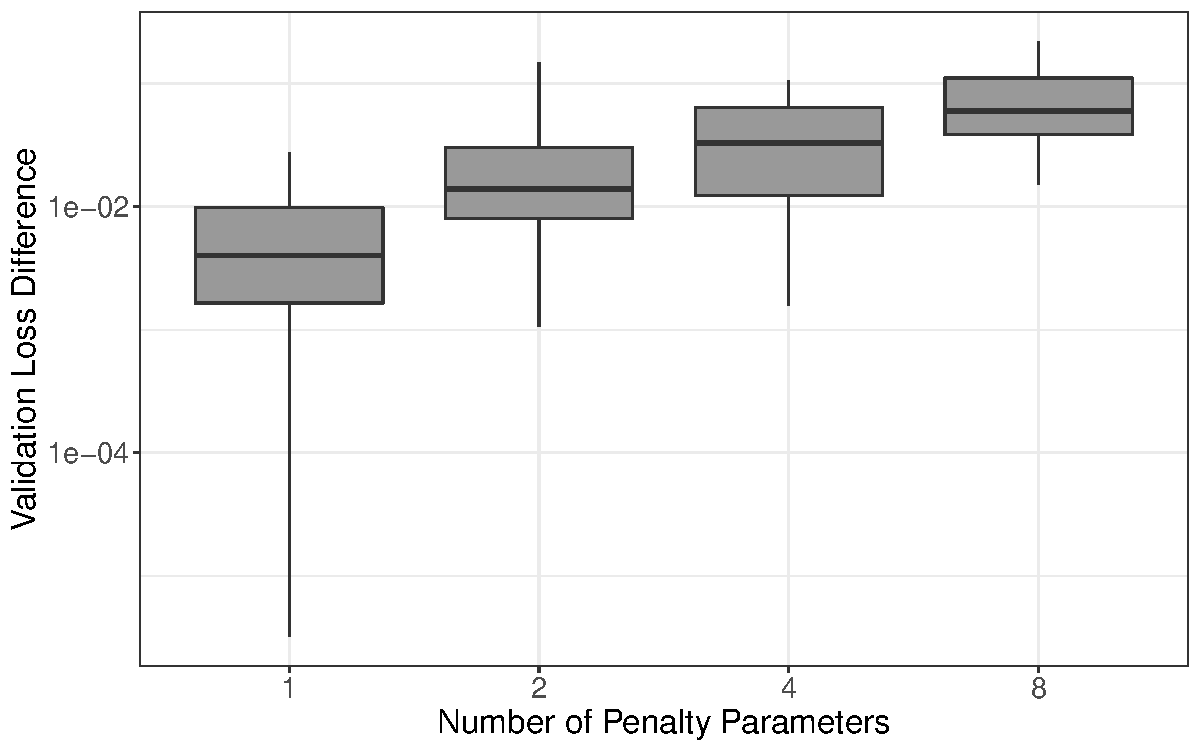
\includegraphics[width=\textwidth]{../../../R/figures/validation_size_loss_diff_homogeneous.pdf}
		\caption{Simulation 1: the univariate additive components are the same}
	\end{subfigure}
	\begin{subfigure}{0.6\textwidth}
		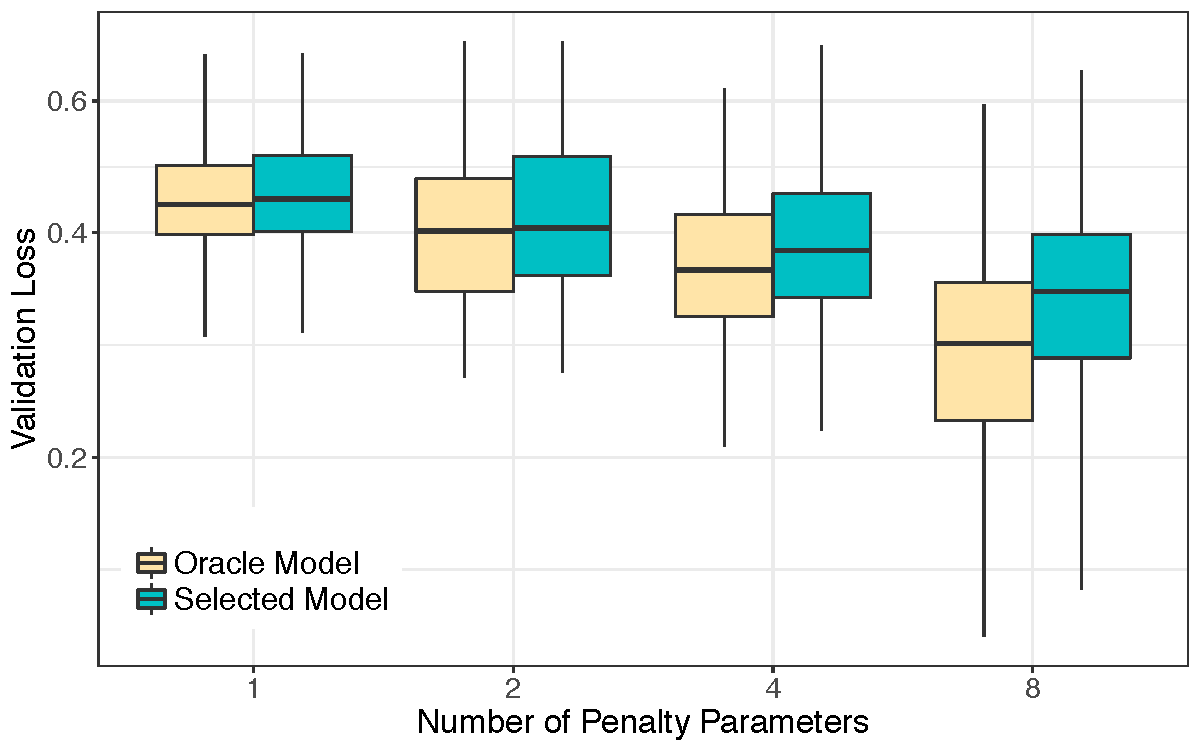
\includegraphics[width=\textwidth]{../../../R/figures/validation_size_loss_heterogeneous_final.pdf}
		\caption{Simulation 2: the univariate additive components have differing levels of smoothness}
	\end{subfigure}
	\caption{
		Performance of generalized additive models as the number of free penalty parameters grows.
	}
	\label{fig:simulations}
\end{figure}

\section{Discussion}\label{sec:discussion}

In this manuscript, we have characterized the generalization error of split-sample procedures that tune multiple hyper-parameters. 
If the estimated models are Lipschitz in the hyper-parameters, the generalization error of the selected model is upper bounded by a combination of the oracle risk and a near-parametric term in the number of hyper-parameters.
These results show that adding hyper-parameters can decrease the generalization error of the selected model if the oracle risk decreases by a sufficient amount.
In the semi- or non-parametric setting, the error incurred from tuning hyper-parameters is dominated by the oracle risk asymptotically; adding hyper-parameters has a negligible effect on the generalization error of the selected model.
In the parametric setting, the error incurred from tuning hyper-parameters is on the same order as the oracle error; one should be careful about adding hyper-parameters, though they are not more ``costly'' than model parameters.

We also showed that many penalized regression examples satisfy the Lipschitz condition so our theoretical results apply.
This implies that fitting models with multiple penalties and penalty parameters can be desirable, rather than the usual case with one or two penalty parameters.

One drawback of our theoretical results is that we have assumed that selected hyper-parameter is a global minimizer of the validation loss.
Unfortunately this is not achievable in practice since the validation loss is not convex with respect to the hyper-parameters.
This problem is exacerbated when there are many hyper-parameters since it is computationally infeasible to perform an exhaustive grid-search. 
We hope to address this question in future research.


%%%%%%%%%%%%%%%%%%%%%%%%%%%%%%%%%%%%%%%%%%%%%%%%%%%%%%%%%%%%%%%%%%%%%%%%%%%%%%%%%%%%%%%%%%%%%%%%%%%%%%%%%%%%%%%%%%%%%%%%%%%%
\vskip 14pt
\noindent {\large\bf Supplementary Materials}

Oracle inequalities for general model-estimation procedures and proofs for all the results are given in the Supplementary Materials.
\par
%%%%%%%%%%%%%%%%%%%%%%%%%%%%%%%%%%%%%%%%%%%%%%%%%%%%%%%%%%%%%%%%%%%%%%%%%%%%%%%%%%%%%%%%%%%%%%%%%%%%%%%%%%%%%%%%%%%%%%%%%%%%
\vskip 14pt
\noindent {\large\bf Acknowledgements}

Jean Feng was supported by NIH grants DP5OD019820 and T32CA206089. Noah Simon was supported by NIH grant DP5OD019820.
\par

\bibliographystyle{unsrtnat}
\bibliography{hyperparam-theory}

\vskip .65cm
\noindent
Jean Feng, Department of Biostatistics, University of Washington
\vskip 2pt
\noindent
E-mail: jeanfeng@u.washington.edu
\vskip 2pt

\noindent
Noah Simon, Department of Biostatistics, University of Washington
\vskip 2pt
\noindent
E-mail: nrsimon@u.washington.edu


\end{document}
